\section{Case Study and Motivation}\label{sec:case_study}

In this section, we will study a particular attention head in Llama 2, and use its behavior as a motivation for the more general analysis that follows.

\subsection{Preliminaries}\label{sub:prelim}

\DP{TODO @TG: Fill out a simplified notation block. Please ensure that the simplified notation is consistent with the notation in the appendix.}

\DP{TODO: mention that we pre-pend all inputs with \bos.}

A significantly more precise setup and notation is detailed in \Cref{sub:app_notation}.

\subsection{Understanding Layer 16 Attention Head 25 of Llama 2}\label{sub:case_study_l25_h16}

As motivation for our later reasoning, we will now examine the behavior of Layer 16 Attention Head 25 (abbreviated as L16H25) in Llama 2 7B, on both prose from the Wikipedia dataset \citep{wikidump} and code from the RedPajama Github dataset \citep{together2023redpajama}. This is the first attention head which we identify as a dormant head, and we want to understand its properties at a more fine-grained level. First, let us examine the difference in perplexity on samples of these two datasets obtained from the full forward pass versus a modified forward pass where the output of the attention head L16H25 is zeroed out. Specifically, we evaluate each forward pass on 32 samples of their respective datasets, where each sample is truncated to 64 tokens. We observe the results in \Cref{tab:ppl_wiki_github_l16h25}. Overall, the performance change is greater on the GitHub data than on the Wikipedia data, which signals that it may be the case that L16H25 is function-less on the Wikipedia data yet has a function on the GitHub data. To confirm our hypothesis, we plot the (post-softmax) attention weights on a few representative samples of GitHub and Wikipedia data in \Cref{fig:attn_l16_h25_small} (and \Cref{fig:attn_l16_h25_improved} in \Cref{sub:app_supporting_lots_of_heads}). We observe that L16H25 is an attention sink \citep{xiao2023efficient} on Wikipedia data. This means that for each sample, the attention head outputs roughly the same vector (or one of a few possible vectors) for each token position, acting like a bias which does not use correlations between tokens. On the other hand, on GitHub data L16H25 is not an attention sink. This discrepancy motivates the definition of a dormant head, expanded on in \Cref{sec:dormant_heads}, that a dormant head is one which does not use correlations between tokens to obtain an output (and thus is not impacted by the semantics of the input). To confirm this, we also plot the pre-softmax logits in \Cref{fig:attn_logits_l16_h25_small} (and \Cref{fig:attn_logits_l16_h25_improved} in \Cref{sub:app_supporting_lots_of_heads}). \DP{TODO: @TG could you give some reasoning here?}

\begin{table}
    \centering
    \caption{\small \textbf{Perplexity of Llama 2 7B when using an unmodified forward pass vs.~a forward pass which is modified to set the output of L16H25 to \(0\).} We observe that while the perplexity does not change substantially on Wikipedia data, it noticeably increases on Github data. This motivates the hypothesis that L16H25 is ``dormant'' for Wikipedia data and ``active'' for Wikipedia data.}
    \begin{tabular}{@{}lll@{}}
    \toprule
    \textbf{Perplexity}    & Wikipedia Dataset & Github Dataset \\ \midrule
    Unmodified forward pass                  &                   &                \\
    Modified forward pass  &                   &                \\ \bottomrule
    \end{tabular} 
    \label{tab:ppl_wiki_github_l16h25}
\end{table}

\begin{figure}
    \centering
    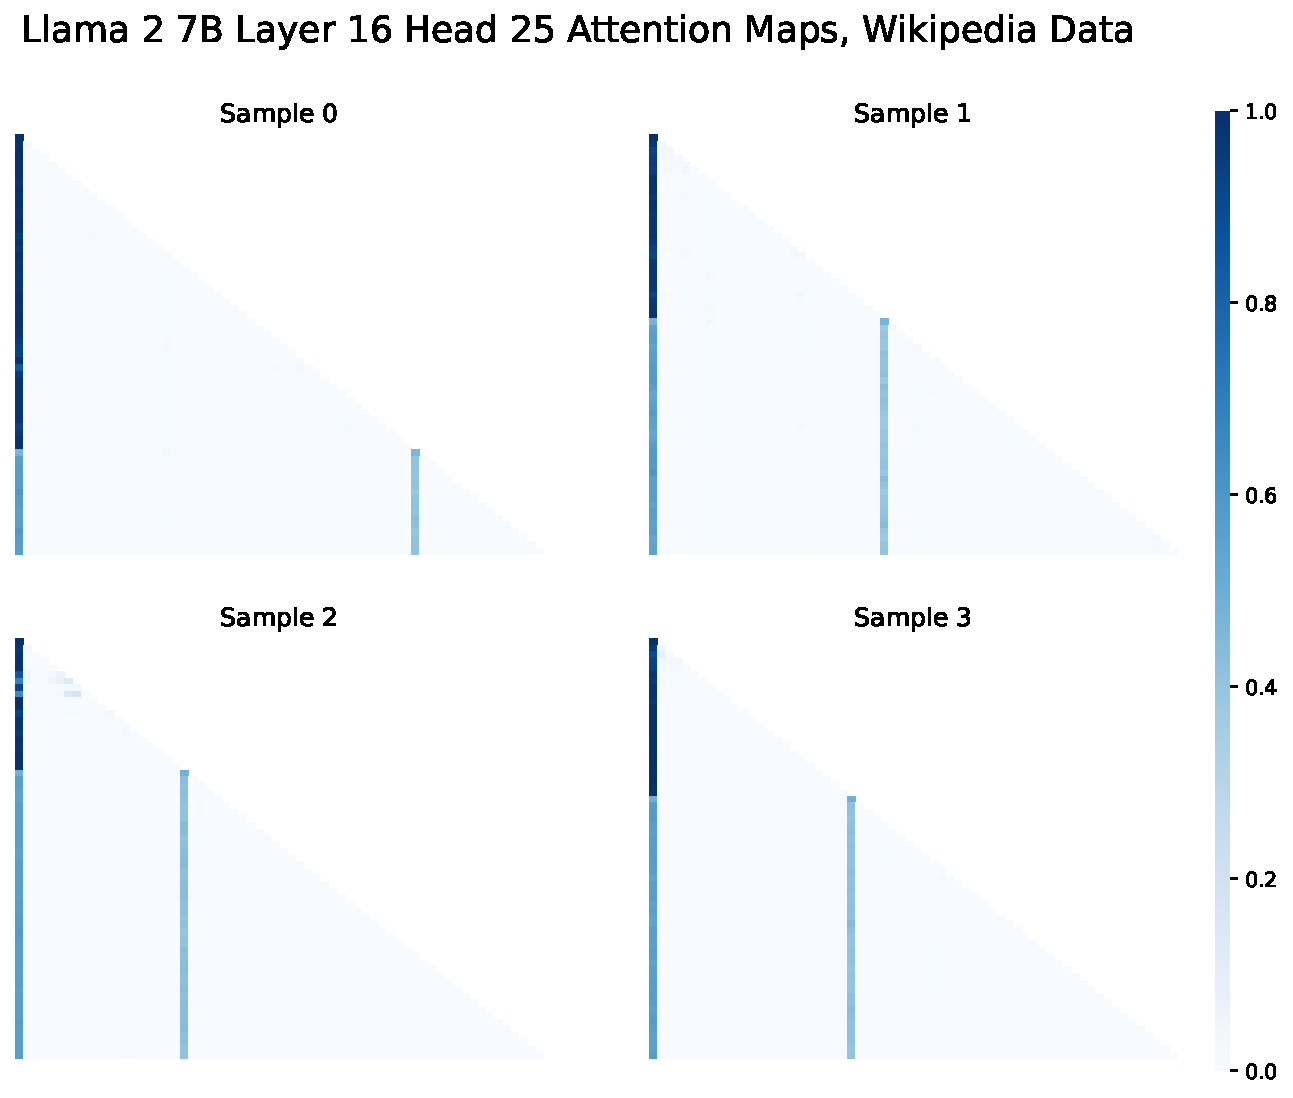
\includegraphics[width=0.45\textwidth]{Figures/L16_H25/attn_maps_l16h25_wiki_small.pdf}
    \hspace{0.075\textwidth}
    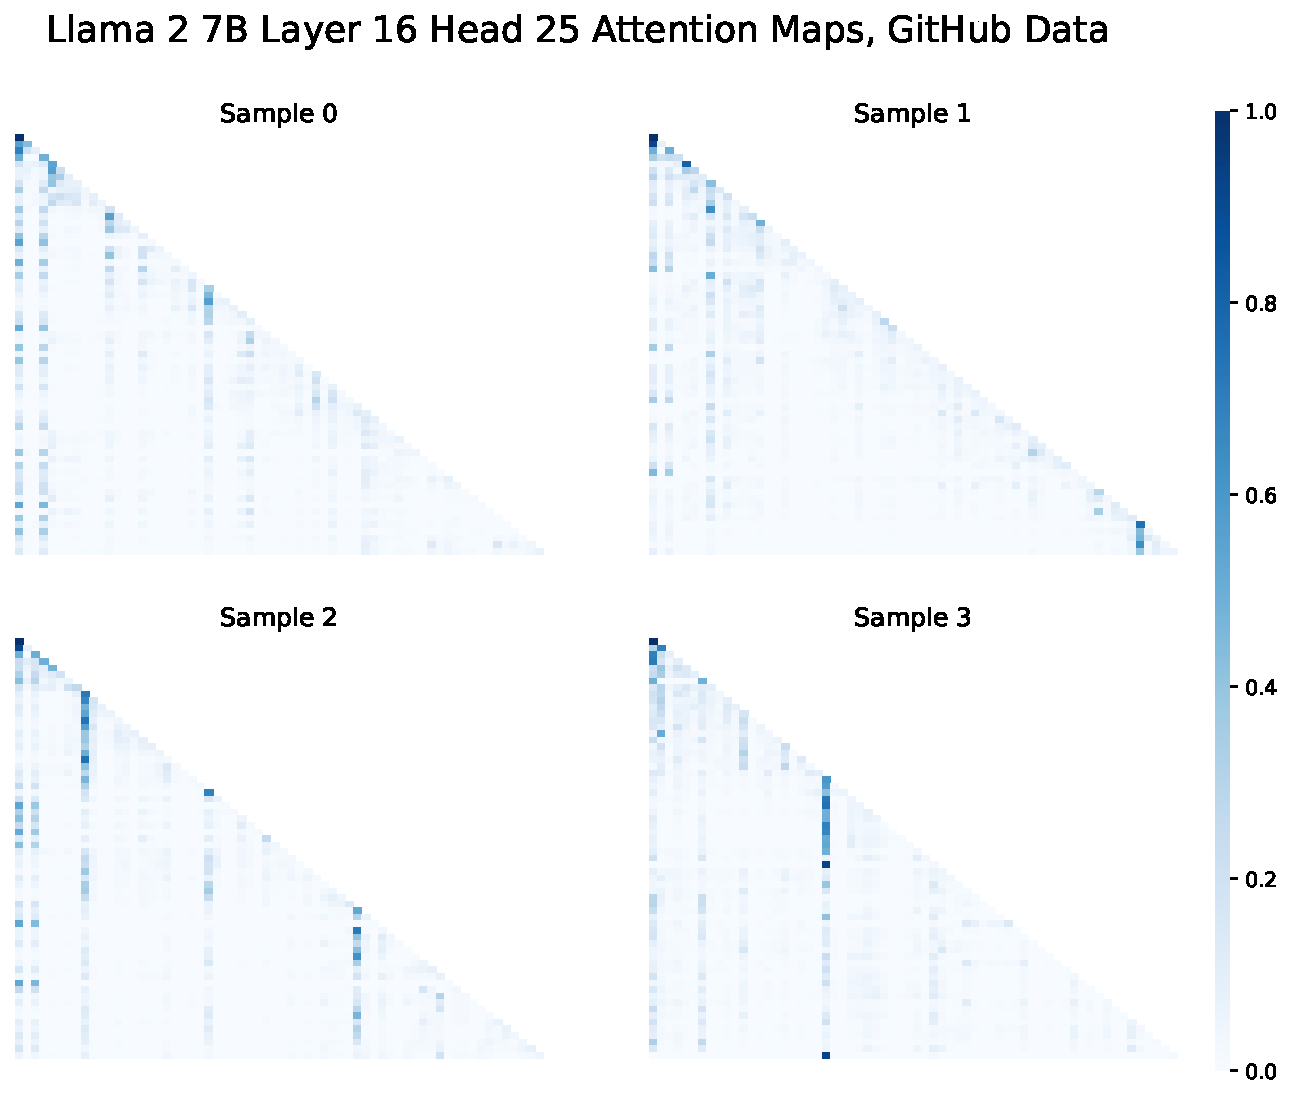
\includegraphics[width=0.45\textwidth]{Figures/L16_H25/attn_maps_l16h25_github_small.pdf}
    \caption{\small\textbf{Visualizations of attention weights for Llama 2 7B L16H25 on both Wikipedia and GitHub data.} On four random samples from each domain, we truncate each sample to 64 tokens and visualize the (post-softmax) attention weights from this head. We observe that for Wikipedia the head has one or two attention sinks, while for GitHub the head has no attention sink, corresponding to our hypothesis that the head is ``dormant'' on Wikipedia and ``active'' on GitHub. Further samples are plotted in \Cref{fig:attn_l16_h25_improved}, maintaining this trend.}
    \label{fig:attn_l16_h25_small}
\end{figure}


\begin{figure}
    \centering
    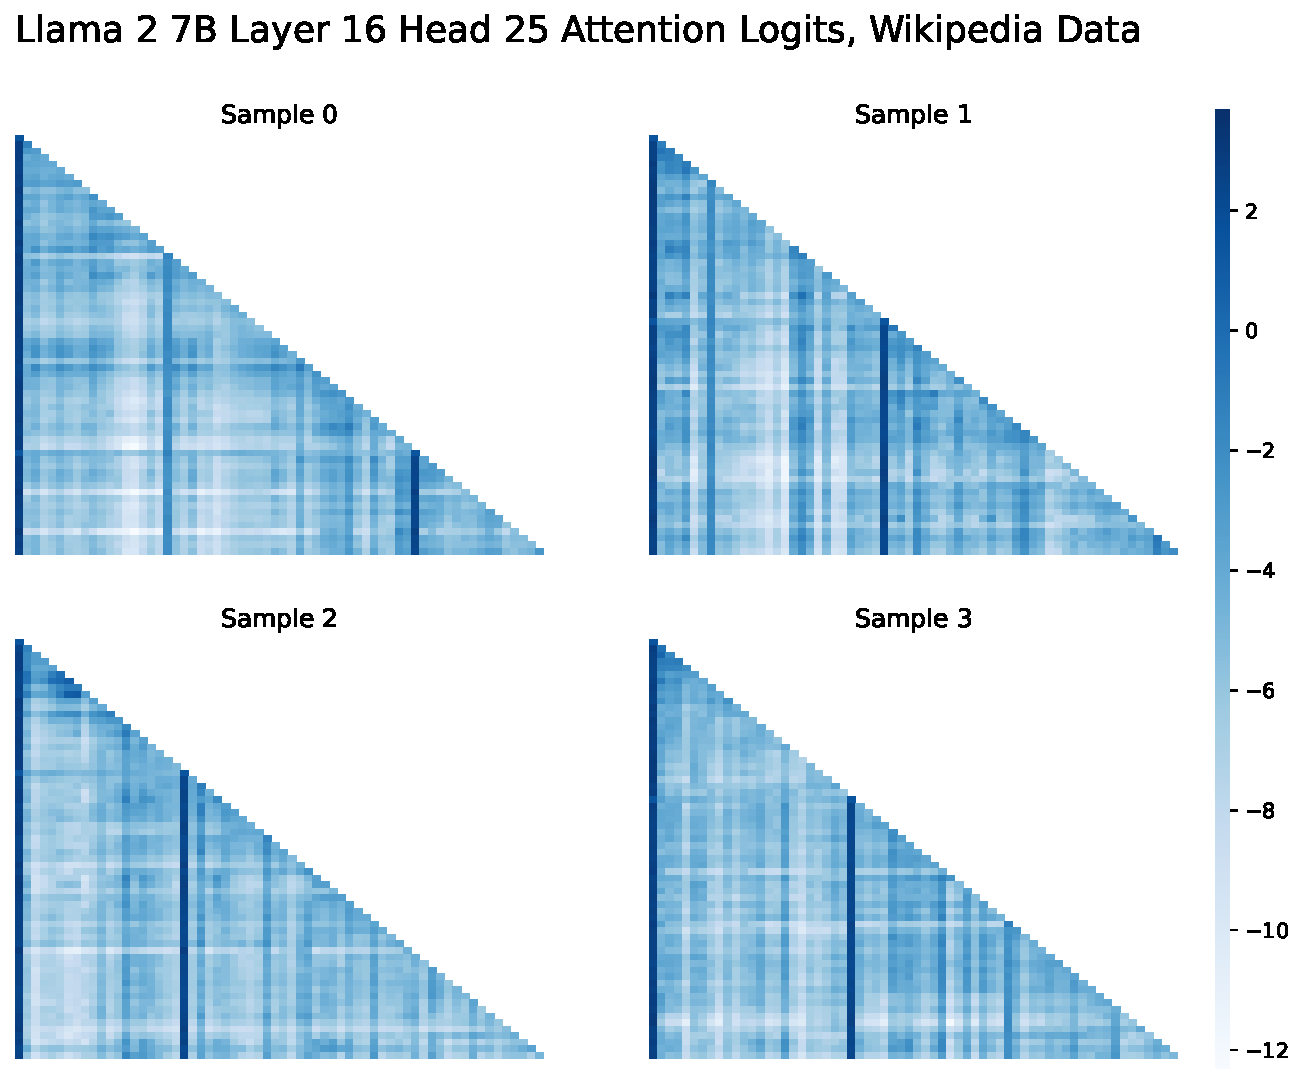
\includegraphics[width=0.45\textwidth]{Figures/L16_H25/attn_logits_l16h25_wiki_small.pdf}
    \hspace{0.075\textwidth}
    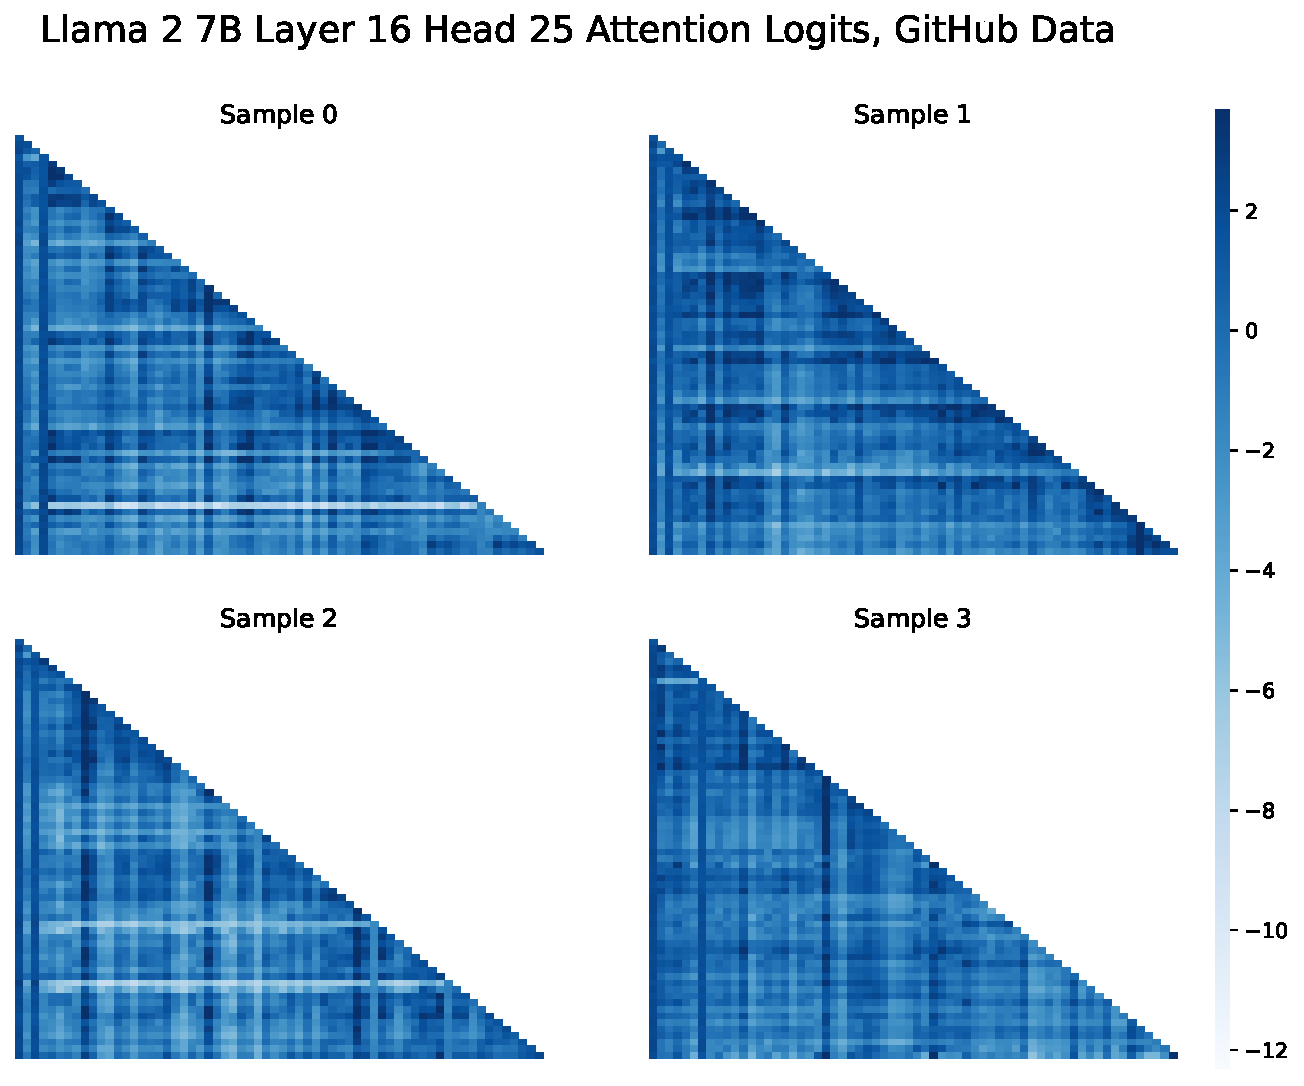
\includegraphics[width=0.45\textwidth]{Figures/L16_H25/attn_logits_l16h25_github_small.pdf}
    \caption{\small\textbf{Visualizations of pre-softmax attention logits for Llama 2 7B L16H25 on both Wikipedia and GitHub data.} \DP{@TG: please fill in the description here and in main body.} Further samples are plotted in \Cref{fig:attn_logits_l16_h25_improved}, maintaining this trend. \tianyu{how about deleting this figure? It's hard to tell that the logits are around the same. Instead, how about make annotations on previous figure, showing the attention logits on bos?}}
    \label{fig:attn_logits_l16_h25_small}
\end{figure}

